% Solution: Tadelis (2013) Exercise 8.7 "Debt and Repayment". Input by \solitem.
% New in the 50-item list. Check: check_D.py.
\begin{exsol}{Tadelis Exercise 8.7}{171}{Advanced}{4}
\asked For the loan game with no courts, free courts and costly courts: the trees and SPE, with
uniqueness ((a), (b), (d)); Nash equilibria that are not SPE ((c), (e)); what the lender would pay
for a ``loser pays the legal fees'' law (f); and whether a planner should adopt it (g).

\method Backward induction with a continuum of actions: for every repayment $x$, solve the
lender's suit decision; then the debtor's choice of $x$; then the lender's offer (Tadelis \S8.1,
Def.~8.1, p.~152; SPE Def.~8.3, p.~157; the Fact on p.~158). Nash equilibria that are not SPE
rely on plans at nodes off the equilibrium path (Def.~7.8, p.~146; \S8.2, pp.~157--158).
Lecture~4: credible and non-credible threats, slides~8, 11 and~13; SPE, slide~17.

\solution
\textbf{Set-up and reading of the statement.} Player~1 (lender, L) chooses $\mathit{Offer}$ or
$\mathit{Not}$. After $\mathit{Offer}$, player~2 (debtor, D) repays $x \in [0, 110]$. Repaying a
negative amount is not an option, so $x \ge 0$. Without a suit, $(u_L, u_D) = (x - 100,\ 110 - x)$.
When courts exist and $x < 105$, the lender then chooses $\mathit{Sue}$ or $\mathit{Not\ sue}$. A suit
brings the total repayment to $105$, with the $x$ already paid counting toward it. The debtor
then pays the fine or the fee on top. The three legal regimes differ only in the payoffs after
$\mathit{Sue}$:
\begin{center}
\begin{tabular}{lccc}
\toprule
& (b) free courts, fine 5 & (d) lender pays fee 105 & (f) debtor pays fee 105 \\
\midrule
$u_L(\mathit{Sue})$ & $105-100 = 5$ & $105 - 100 - 105 = -100$ & $105-100 = 5$ \\
$u_D(\mathit{Sue})$ & $110 - 105 - 5 = 0$ & $110 - 105 - 5 = 0$ & $110 - 105 - 105 = -100$ \\
\bottomrule
\end{tabular}
\end{center}
\begin{center}
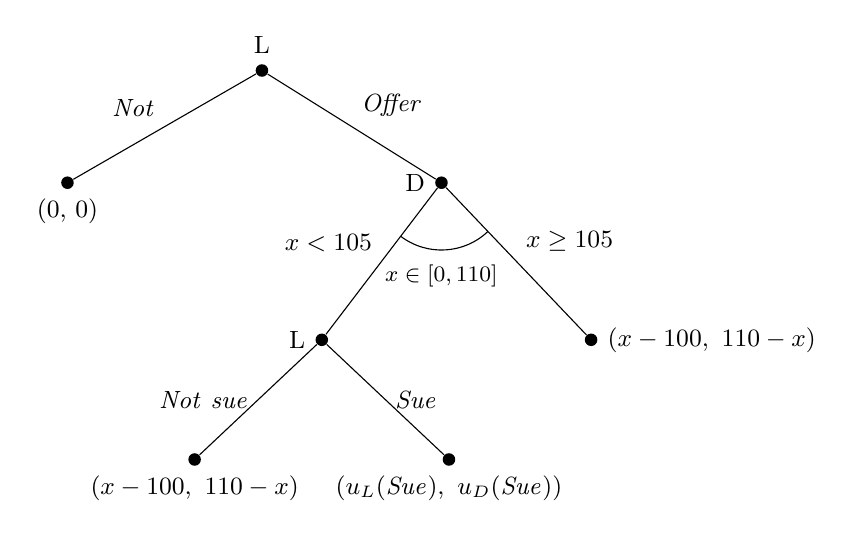
\begin{tikzpicture}[scale=0.95,dot/.style={circle,fill,inner sep=1.6pt},
  every node/.style={font=\small}]
  \node[dot,label=above:{L}] (r) at (0,0) {};
  \node[dot,label=below:{$(0,\,0)$}] (n) at (-2.6,-1.5) {};
  \node[dot,label=left:{D}] (d) at (2.4,-1.5) {};
  \draw (r) -- node[above left] {$\mathit{Not}$} (n);
  \draw (r) -- node[above right] {$\mathit{Offer}$} (d);
  \node[dot,label=left:{L}] (s) at (0.8,-3.6) {};
  \node[dot,label=right:{$(x-100,\ 110-x)$}] (x1) at (4.4,-3.6) {};
  \draw (d) -- node[above left] {$x < 105$} (s);
  \draw (d) -- node[above right] {$x \ge 105$} (x1);
  \draw (d) ++(-127.3:0.9) arc[start angle=-127.3,end angle=-46.4,radius=0.9];
  \node[font=\footnotesize] at (2.4,-2.75) {$x \in [0,110]$};
  \node[dot,label=below:{$(x-100,\ 110-x)$}] (ns) at (-0.9,-5.2) {};
  \node[dot,label=below:{$(u_L(\mathit{Sue}),\ u_D(\mathit{Sue}))$}] (su) at (2.5,-5.2) {};
  \draw (s) -- node[left] {$\mathit{Not\ sue}$} (ns);
  \draw (s) -- node[right] {$\mathit{Sue}$} (su);
\end{tikzpicture}\\[2pt]
{\footnotesize Payoffs $(u_L,u_D)$. The arc marks the continuum of repayments $x$. The lender's node
after $x<105$ exists only in (b), (d) and (f); in (a) every $x$ ends the game with
$(x-100, 110-x)$.}
\end{center}
A pure strategy of the lender is an offer decision plus a suit rule $\mathit{sue}(x)$ for every
$x < 105$: a function, not a single choice. A pure strategy of the debtor is a number $x$.

\textbf{(a) No legal system.} \emph{Debtor:} $110 - x$ is strictly decreasing, so $x^* = 0$, giving
$(u_L, u_D) = (-100, 110)$. \emph{Lender:} $\mathit{Not}$ gives $0 > -100$. SPE:
$(\mathit{Not};\ x = 0)$, payoffs $(0,0)$. It is unique, since both maximizers are unique.

\textbf{(b) Costless courts.} \emph{Lender after a default $x<105$:} $\mathit{Sue}$ gives $5 > x - 100$,
so he sues after every default. \emph{Debtor:} any $x<105$ is followed by a suit and gives $0$;
$x \in [105, 110]$ gives $110 - x \le 5$, with the maximum at $x = 105$. Since $5 > 0$, $x^* = 105$.
\emph{Lender at the root:} $\mathit{Offer}$ gives $105 - 100 = 5 > 0$. SPE:
\[
  \bigl(\mathit{Offer},\ \mathit{sue}(x) = \mathit{Sue}\ \forall x < 105;\ \ x = 105\bigr),
  \qquad (u_L,u_D) = (5,5).
\]
It is unique: every comparison is strict and $x = 105$ is the only maximizer.

\textbf{(c) Nash equilibria of (b) that are not SPE: none in pure strategies.}
\begin{itemize}
  \item \emph{No pure NE without lending.} Whatever $x$ the debtor plans, the lender can switch to
  $\mathit{Offer}$ and to a suit rule that is best at that $x$. He then gets $5$ if $x < 105$ (sue)
  or $x - 100 \ge 5$ if $x \ge 105$, more than $0$. So $\mathit{Not}$ is never a best reply. Unlike a threat
  against the opponent, a lender's plan ``I would not sue'' cannot keep him out: he controls it.
  \item \emph{With lending, the profile is forced.} If $x > 105$ the debtor gains by moving to
  $105$. If $x < 105$ the lender gains by suing (if he does not) or the debtor gains by moving to
  $105$ (if he does: $5 > 0$). So $x = 105$. If the suit rule skipped even one $x' < 105$, the
  debtor would move there and get $110 - x' > 5$. So the rule must be ``sue after every
  $x' < 105$'', which is the SPE.
\end{itemize}
So in pure strategies the only Nash equilibrium is the SPE. With behavioural strategies the answer
changes, though not the outcome. The lender may randomize at unreached defaults and sue after
$x'$ with probability $s(x')$, provided the debtor still prefers $105$:
$(1 - s(x'))(110 - x') \le 5$, i.e.\ $s(x') \ge 1 - \frac{5}{110 - x'}$ (e.g.\ $\frac16$ at
$x' = 104$). Any $s(x') < 1$ is not sequentially rational, since suing is strictly better. These are
Nash equilibria that are not SPE, with the same path and payoffs $(5,5)$.

\textbf{(d) Costly courts (lender pays the fee).} \emph{Lender after a default $x < 105$:}
$\mathit{Sue}$ gives $-100$ and $\mathit{Not\ sue}$ gives $x - 100$. Not suing is strictly better for
every $x > 0$, and at $x = 0$ the two tie ($-100 = -100$). \emph{Debtor:} if the lender does not sue at
$x = 0$, the debtor's payoff $110 - x$ on $[0,105)$ is maximized at $x = 0$, giving $110$, which beats
$110 - x \le 5$ on $[105,110]$. Could the lender instead sue at $x=0$, with probability $s > 0$? The
debtor would get $110(1 - s) < 110$ at $x = 0$ and $110 - x$ at every small $x > 0$. The supremum
$110$ is then not attained, so the debtor has no best reply. The tie at $0$ must therefore be broken
toward $\mathit{Not\ sue}$. \emph{Lender at the root:} $\mathit{Offer}$ gives $-100 < 0$. The unique SPE
is
\[
  \bigl(\mathit{Not},\ \mathit{sue}(x) = \mathit{Not\ sue}\ \forall x<105;\ \ x = 0\bigr),
  \qquad (u_L,u_D) = (0,0),
\]
the outcome of (a). A legal system that is too expensive to use is the same as none.

\textbf{(e) Nash equilibria of (d) that are not SPE: yes.}
\begin{itemize}
  \item \emph{Lending supported by a non-credible threat:}
  \[
    \bigl(\mathit{Offer},\ \mathit{sue}(x) = \mathit{Sue}\ \forall x < 105;\ \ x = 105\bigr),
    \qquad (u_L,u_D) = (5,5).
  \]
  It is a NE. The debtor gets $5$ at $x = 105$ and $0$ at any default, since he is sued. The lender
  gets $5 > 0$, and no suit node is reached, so the suit rule costs him nothing. It is not an SPE.
  In the subgame after any default $x > 0$, suing gives $-100 < x - 100$. As in (c), this is the
  only NE with lending in pure strategies: one gap in the suit rule invites the debtor to default
  there. It is better for \emph{both} players than the SPE $(0,0)$. The threat is what would make
  lending possible, but it is not credible.
  \item \emph{No lending, with other plans:} $\mathit{Not}$, any planned $x \le 100$ and any suit
  decision at that $x$. Offering would give the lender at most $\max\{-100,\ x - 100\} = x - 100
  \le 0$. All of these except the SPE are Nash equilibria that are not subgame perfect, e.g.\
  $(\mathit{Not},\ \text{never sue};\ x = 50)$, because $x = 50$ is not the debtor's best reply after
  $\mathit{Offer}$.
\end{itemize}

\textbf{(f) Loser pays the fees.} After a default $x<105$, $\mathit{Sue}$ gives the lender
$105 - 100 = 5 > x - 100$: the suit is now credible. The debtor gets $-100$ from any default and
$110 - x$ from $x \in [105,110]$, so $x = 105$ ($5 > -100$). Offering gives $5 > 0$. Unique SPE:
$(\mathit{Offer},\ \mathit{Sue}\ \forall x<105;\ x = 105)$, payoffs $(5,5)$. Compared with (d) the
lender's equilibrium payoff rises from $0$ to $5$. Anything he pays for the reform is sunk before the
game starts and does not change the SPE, so he gains iff the price is below \$5. He would pay
\emph{up to \$5}.

\textbf{(g) The planner.} Total surplus is $0$ without the law (no loan) and $110 - 100 = 10$ with it.
On the equilibrium path nobody defaults, so nobody is sued and the \$105 fee is never paid. The
reform moves both players from $(0,0)$ to $(5,5)$, a Pareto improvement, so the planner should adopt
it if enacting it costs less than \$10 (the debtor too would pay up to \$5). The harsh off-path
penalty ($-100$ for the debtor) has no social cost in this model because it is never imposed. It
would have one if default could happen by bad luck, which the model rules out.

\interp The project creates \$10 of value, but the lender can capture it only if the debtor
believes default will be punished. In (a) and (d) the debtor's promise to repay is not credible,
and in (d) neither is the lender's threat to sue, because a suit costs more than it recovers.
Lending collapses even though both would gain. The Nash equilibrium in (e) shows the gains a
credible threat would deliver. The SPE shows why the threat by itself does not work. The reform in (f) does not change what happens
on the path; it changes who pays for enforcement \emph{off} the path. That makes suing the
lender's best reply to default, so the threat becomes credible and is never used. This is the
Brexit lesson in a credit market (slides~11 and~13): the institution that makes a threat credible
creates value, while announcing the threat creates none. Free courts in (b) and loser-pays in (f)
give the same outcome.

\verify \texttt{check\_D.py} encodes the payoffs of the four regimes exactly and works on the
repayment grid $x \in \{k/8\}$, which contains $0$, $100$, $104.5$ and $105$. It computes the
sequentially rational suit choice at every default, showing the tie at $x=0$ in (d) and strict
preferences elsewhere. It then computes the debtor's best $x$ and the lender's offer. It tests
the claimed Nash equilibria with unilateral deviations: the lender's joint offer/suit deviations
and every debtor $x$. It confirms that a single gap in the suit rule breaks the threat equilibria
and that no no-lending NE exists in (b). It also checks the behavioural bound
$s(x') \ge 1 - \frac5{110 - x'}$. Output: ``Tadelis 8.7: (a) no loan, x = 0, (0,0); (b) loan, x =
105, sue every x < 105, (5,5); (c) pure NE = SPE; (d) no loan, x = 0, never sue (tie at x = 0), (0,0);
(e) NE with loan and threat to sue, (5,5), and no-loan NE with x <= 100; (f) lender pays up to 5;
(g) surplus +10''. Tadelis prints no answer.

\mistakes
\begin{itemize}
  \item Reading (c) as ``the lender threatens not to sue, so he does not lend''. The lender's own off-path
  plan cannot discipline the lender: he can change his whole strategy, offer and suit rule
  together. In (b) every Nash equilibrium in pure strategies lends.
  \item In (d), leaving the tie at $x=0$ unresolved, or claiming an SPE where the lender sues only at
  $x = 0$. Then the debtor has no best reply, so that profile cannot be part of an equilibrium.
  \item In (f) and (g), counting the \$105 fee as a cost of the reform. It is paid only after a
  default, which never happens in equilibrium.
\end{itemize}

\answer{(a) SPE $(\mathit{Not};\ x = 0)$, payoffs $(0,0)$, unique. (b) SPE: offer, repay $x = 105$,
sue after every $x < 105$; payoffs $(5,5)$, unique. (c) None in pure strategies: the only pure
Nash equilibrium is the SPE (behavioural NE with off-path suit probability
$s(x') \in [1 - \frac{5}{110-x'}, 1)$ exist, with the same outcome). (d) SPE: no loan, $x = 0$, never
sue; payoffs $(0,0)$, unique (the tie at $x = 0$ must go to not suing). (e) Yes: (offer, sue after
every default; $x = 105$), payoffs $(5,5)$, rests on a non-credible threat to sue; so do the other no-loan
profiles with planned $x \le 100$. (f) Yes, up to \$5 (his SPE payoff goes from 0 to 5). (g) Yes:
surplus rises from 0 to 10, both gain \$5, and the fee is never paid in equilibrium.}
\end{exsol}
